

\chapter{Sprint 5}
\label{Sprint0}
\lhead{Chapter 11. \emph{Sprint 5}}

\section{Goal(s)}

This was the final sprint of our project. Its main goal was to
finalize the product and the documentation as well as prepare
a presentation.

\section{Duration}
The duration of the sprint was the following:
\begin{itemize}
\item Sprint start:  November, 4th
\item Milestone M3 (feature freeze): November, 4th.
\item Sprint end: November, 20th
\end{itemize}

\begin{figure}[h]
\centering
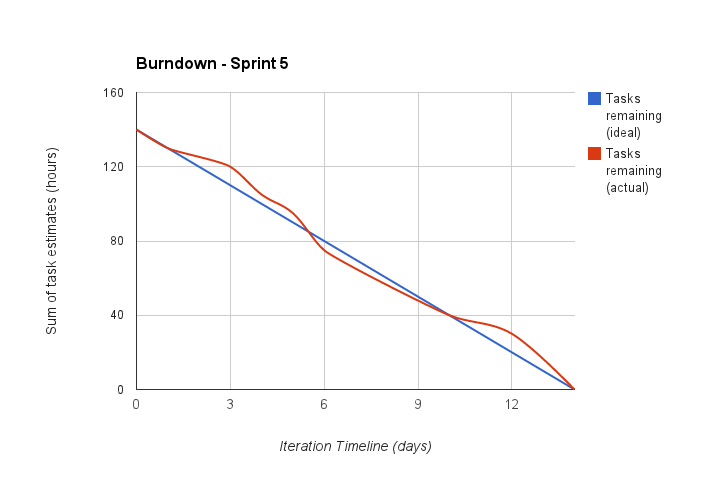
\includegraphics[scale=0.60]{../Figures/burndownSprint5.png}
\caption{Burndown chart Sprint 5}
\label{figure:burndownsprint5}
\end{figure}

This sprint was a bit longer than the others because it included the last days
that were left till the end project.

\section{Planning}

The plan for this sprint consisted primarily in report writing and review.
At the beginning of the sprint we agreed with the supervisor to deliver him a mostly
finished version of the report by the end of the first week in order to let him
give us some last feedback on it.

\section{Backlog}
See below the sprint backlog.
\begin{enumerate}[1.]
\item a
\end{enumerate}

\section{Results and feedback}

from customer, from supervisor
\section{Evaluation}
our thoughts about this sprint